% -*- mode: noweb; noweb-default-code-mode: R-mode; -*-
% \VignetteIndexEntry{An R Package for Ordinal Response Modeling in High-Dimensions} 
% \VignetteKeyword{models}
%% no need \usepackage{Sweave.sty}
\documentclass[article, shortclass, nojss]{jss}
\usepackage{amsmath, graphicx}
\usepackage[superscript,biblabel]{cite}
\title{A tutorial on fitting ordinal response models in high-dimensional datasets with the\pkg{ordinalgmifs} package}
\author{Kellie J. Archer$^\star$,  Jiayi Hou$^b$, Qing Zhou$^\star$,  Kyle Ferber$^\star$,  John G. Layne$^\star$,  Amanda Gentry$^\star$\\
$^\star$ Virginia Commonwealth University,
$^b$ University of California San Diego}
\newcommand{\bet}{\mbox{\boldmath $\beta$}}
\newcommand{\gambold}{\mbox{\boldmath $\gamma$}}
\newcommand{\pibold}{\mbox{\boldmath $\pi$}}
\newcommand{\phibold}{\mbox{\boldmath $\phi$}}
\newcommand{\thetabold}{\mbox{\boldmath $\theta$}}
\newcommand{\nubold}{\mbox{\boldmath $\nu$}}
\newcommand{\taubold}{\mbox{\boldmath $\tau$}}
\newcommand{\alphabold}{\mbox{\boldmath $\alpha$}}
\newcommand{\wbold}{\boldsymbol{w}}
\Plainauthor{Kellie J Archer, Jiayi Hou, Qing Zhou, Kyle Ferber, John G. Layne, Amanda Gentry}
\Plaintitle{ordinalgmifs: An R Package for Ordinal Regression in High-dimensional Data Settings}
\Shorttitle{High-dimensional Ordinal Response Models}

\Abstract{In this tutorial we describe our \pkg{ordinalgmifs} \proglang{R} package, available from the Comprehensive R Archive Network, that can fit a variety of ordinal response models when the number of predictors ($P$) exceeds the sample size ($n$).  We then illustrate the functions in the \pkg{ordinalgmifs} \proglang{R} package using a dataset where we were interested in predicting normal $<$ pre-neoplastic $<$ neoplastic states of liver disease using a subset of CpG sites from a high-throughout methylation assay \cite{ArcherHCC}.  
}
\Keywords{ordinal response, high-dimensional features, penalized models, \proglang{R}}
\Plainkeywords{ordinal response, high-dimensional features, penalized models, R}

\Address{
Kellie J. Archer\\
Department of Biostatistics\\
Virginia Commonwealth University\\
Box 980032\\
Richmond, VA 23298-0032\\
E-mail: \email{kjarcher@vcu.edu}\\
URL: \url{http://www.people.vcu.edu/~kjarcher/}\\
 \\
Jiayi Hou\\
Clinical and Translational Research Institute\\
University of California San Diego\\
San Diego, CA\\
E-mail: \email{jhou@ucsd.edu}\\
\\
Qing Zhou\\
Department of Biostatistics\\
Virginia Commonwealth University\\
Box 980032\\
Richmond, VA 23298-0032\\
E-mail: \email{zhouq3@mymail.vcu.edu}\\
\\
Kyle Ferber\\
Department of Biostatistics\\
Virginia Commonwealth University\\
Box 980032\\
Richmond, VA 23298-0032\\
E-mail: \email{ferberkl@mymail.vcu.edu}\\
\\
John G. Layne\\
Center fo the Study of Biological Complexity\\
Virginia Commonwealth University\\
Box 842537\\
Richmond, VA 23298\\
E-mail: \email{laynejg@vcu.edu}\\
\\
Amanda Gentry\\
Department of Biostatistics\\
Virginia Commonwealth University\\
Box 980032\\
Richmond, VA 23298-0032\\
E-mail: \email{gentryae@mymail.vcu.edu}\\
}

\usepackage{a4wide}

\begin{document}

%\maketitle
\section{Introduction}
Various algorithms can be used for obtaining solutions for the Least Absolute Shrinkage and Selection Operator (LASSO) \cite{Tibs1996, Tibs1997} and elastic net penalized models \cite{Zou}. In the linear regression setting, the Incremental Forward Stagewise (IFS) is a penalized solution that enforces monotonicity \cite{Hastie}. IFS can be generalized to problems involving other than squared error loss, and the adaption is called the generalized monotone incremental forward stagewise (GMIFS) method \cite{Hastie}. Herein we extended the GMIFS method  \cite{Hastie} to ordinal response setting and implemented various functions in our \pkg{ordinalgmifs} \proglang{R} package. The \code{ordinal.gmifs} function can be used to fit traditional and penalized cumulative link, forward continuation ratio, and backward continuation ratio models using either a logit, probit, or complementary log-log link. It can also be used to fit adjacent category and stereotype logit models. A detailed description of the methodology is available in \cite{ArcherCI}.

\section{Implementation}
The \pkg{ordinalgmifs} package was written in the \proglang{R} programming environment \cite{RTeam}.  The \code{ordinal.gmifs} function allows the user to specify a model formula, identify the matrix of covariates to be penalized in the model fitting algorithm using the \code{x} parameter, and additionally specify the model type (\code{probability.model}) and link function (\code{link}). The default is to fit a cumulative logit model though allowable probability models include \code{"Cumulative"}, \code{"ForwardCR"}, \code{"BackwardCR"}, \code{"AdjCategory"}, and \code{"Stereotype"} while allowable links include \code{"logit"}, \code{"probit"}, \code{"cloglog"} for the first three and \code{"loge"} and \code{"logit"} for the last two, respectively. The defaults for updating the penalized coefficients are \code{epsilon=0.001} and \code{tol=1e-5}. Our likelihood functions were written in \proglang{R} and  tested by comparing our \proglang{R} output to output produced by the \code{vglm} \proglang{R} \pkg{VGAM} package for cumulative link, adjacent category, forward and backward continuation ratio models and to \proglang{STATA}'s \texttt{slogit} function and the \code{rrvglm} function in the \proglang{R} \pkg{VGAM} for the stereotype logit model using benchmark datasets for data where $P<n$.

\section{Examples}
The \pkg{ordinalgmifs} package includes example datasets having an ordinal response. These data are a subset of subjects and CpG sites reported in the original paper where liver samples were assayed using the Illumina GoldenGate Methylation BeadArray Cancer Panel I \cite{ArcherHCC}. Technical replicate samples and matched cirrhotic samples from subjects with hepatocellular carcinoma (HCC) were removed to ensure all samples were independent. For the following examples, methylation levels for 45 CpG sites in liver tissue are provided for independent subjects whose liver was either Normal (N=20), cirrhotic but not having HCC (N=16, Cirrhosis non-HCC), and HCC (N=20, Tumor). These data are in two formats: a \code{data.frame} (\code{hccframe}) and as a BioConductor \code{ExpressionSet} (\code{hccmethyl}). We seek to predict \code{group} which indicates sample type (\code{Normal} < \code{Cirrhosis non-HCC} < \code{Tumor}) using the CpG site methylation values as predictor variables. 
 
\subsection{Model Fitting for Data Stored in a data.frame}
To fit a model where all predictors are penalized the model formula is specified to fit an intercept only model and the predictors to be penalized are specified using the \code{x} parameter. When fitting a penalized model it is expected that more than one variable is included in the \code{x} parameter. The \code{x} parameter can either be a vector naming columns in the \code{data.frame} specified by the \code{data} parameter or \code{x} can be a the \code{data.frame} name with the columns to include (or exclude) indicated by their (negative) index. Prior to model fitting \code{NA} values should be imputed or removed from the \code{data.frame}. By default a cumulative logit model is fit when neither \code{probability.model} nor \code{link} are specified by the user. Because \code{group} is the first variable in the \code{hccframe}, we fit a model penalizing all CpG sites by specifying \code{x=hccframe[,-1]} which simply removes our ordinal outcome.
\begin{Schunk}
\begin{Sinput}
> library("ordinalgmifs")
> data(hccframe)
> cumulative.logit<-ordinal.gmifs(group ~ 1, x = hccframe[,-1], 
+ 	data = hccframe)
\end{Sinput}
\end{Schunk}
Because the GMIFS procedure is incremental, the user may want to specify \code{verbose=TRUE} to print the step number in order to monitor the status of the model fitting procedure.

Methods including \code{coef}, \code{plot}, \code{predict}, \code{fitted}, \code{print}, and \code{summary} can be applied to \code{ordinalgmifs} model objects. Because the returned list differs depending on whether a no penalty subset is included or a stereotype logit model is fit, the \code{print} function returns the object names of the fitted object. 
\begin{Schunk}
\begin{Sinput}
> print(cumulative.logit)
\end{Sinput}
\begin{Soutput}
 [1] "beta"              "alpha"             "zeta"             
 [4] "x"                 "y"                 "w"                
 [7] "scale"             "logLik"            "AIC"              
[10] "BIC"               "model.select"      "probability.model"
[13] "link"             
\end{Soutput}
\end{Schunk}
By default \code{coef}, \code{predict}, and \code{summary} extracts the relevant information from the step in the solution path that attained the minimum AIC.
\begin{Schunk}
\begin{Sinput}
> summary(cumulative.logit)
\end{Sinput}
\begin{Soutput}
Cumulative model using a  logit  link 
at step    =  15062 
logLik     =  -1.5684 
AIC        =  138315 
BIC        =  151280 

       (Intercept):1        (Intercept):2 CDKN2B_seq_50_S294_F 
             -5.1727               4.9504              -1.2870 
       DDIT3_P1313_R          ERN1_P809_R           GML_E144_F 
             -1.2830               0.3620               1.9060 
        HDAC9_P137_R      HLA.DPA1_P205_R         HOXB2_P488_R 
              0.0830               0.3540              -0.0760 
         IL16_P226_F           IL16_P93_R            IL8_P83_F 
              1.8050               0.3380               0.3810 
          MPO_E302_R           MPO_P883_R        PADI4_P1158_R 
              0.7150               0.1710              -0.9420 
        SOX17_P287_R          TJP2_P518_F            WRN_E57_F 
             -1.9250              -2.0230               0.5300 
        CRIP1_P874_R       SLC22A3_P634_F         CCNA1_P216_F 
              0.0000               0.0000               0.0000 
        SEPT9_P374_F         ITGA2_E120_F         ITGA6_P718_R 
              0.0000               0.0000               0.0000 
         HGF_P1293_R          DLG3_E340_F             APP_E8_F 
              0.0000               0.0000               0.0000 
        SFTPB_P689_R          PENK_P447_R          COMT_E401_F 
              0.3000               0.0000               0.5810 
       NOTCH1_E452_R         EPHA8_P456_R           WT1_P853_F 
              0.0000               0.0000               0.0000 
        KLK10_P268_R         PCDH1_P264_F         TDGF1_P428_R 
              0.0000               0.0000               0.0000 
        EFNB3_P442_R         MMP19_P306_F         FGFR2_P460_R 
              0.0000               0.0000               0.0000 
         RAF1_P330_F         BMPR2_E435_F         GRB10_P496_R 
              0.0000               0.0000               0.0000 
         CTSH_P238_F SLC6A8_seq_28_S227_F        PLXDC1_P236_F 
              0.0000               0.0000               0.0000 
         TFE3_P421_F        TSG101_P139_R 
              0.0000               0.0000 
\end{Soutput}
\end{Schunk}
However, any step along the solution path can be extracted by specifying the step using the \code{model.select} parameter for these three functions. For example, the model attaining the minimum BIC can be extracted using 
\newline \code{summary(cumulative.logit, model.select=which.min(cumulative.logit$BIC))}. \newline Alternatively, the 150$^{th}$ step can be extracted using \newline \code{summary(cumulative.logit, model.select=150)}. \newline Note that the $\alpha_j$ thresholds are labelled as \code{(Intercept):1},$\ldots$,\code{(Intercept):K-1}.

The \code{plot} function plots the solution path of the model fit. The vertical axis can be changed using the \code{type} parameter with allowable selections being \code{"trace"} (default), \code{"AIC"}, \code{"BIC"} or \code{"logLik"}. Although there are default x-axis, y-axis, and titles provided for each plot, the user can modify these by supplying their own arguments to \code{xlab}, \code{ylab}, and \code{main}, respectively.
\begin{figure}[h]
  \begin{center}
\begin{Schunk}
\begin{Sinput}
> plot(cumulative.logit)
\end{Sinput}
\end{Schunk}
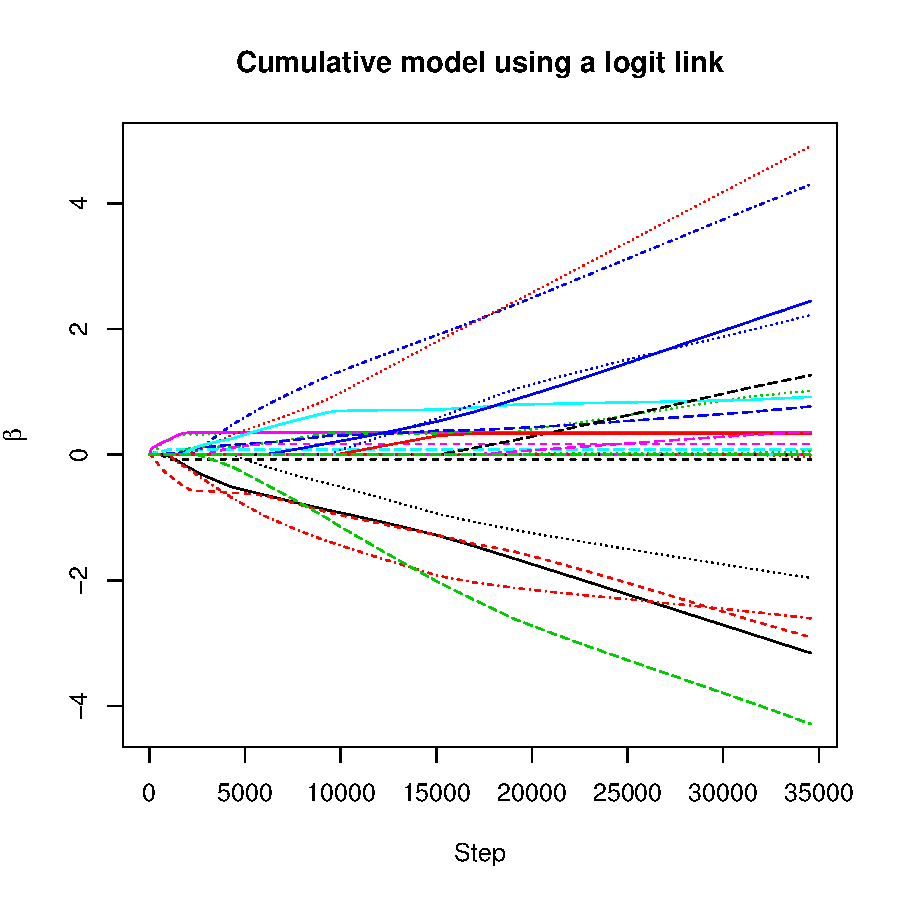
\includegraphics{ordinalgmifs-005}
    \caption{Coefficient estimates along the solution path for a fitted \code{ordinalgmifs} object using the \code{hccframe} data.}
  \end{center}
\end{figure}

The \code{predict} function (or equivalently, \code{fitted}) returns a list containing \code{predicted}, a matrix of the class probabilities from the fitted model, and \code{class}, the class having the maximum predicted probability from the fitted model. As with \code{coef} and \code{summary} the \code{predict} function by default extracts the model that attained the minimum AIC, but predictions for any step along the solution path can be obtained by specifying the step using the \code{model.select} parameter. 

\begin{Schunk}
\begin{Sinput}
> phat <- predict(cumulative.logit)
> table(phat$class, hccframe$group)
\end{Sinput}
\begin{Soutput}
                    Normal Cirrhosis non-HCC Tumor
  Normal                20                 0     0
  Cirrhosis non-HCC      0                16     0
  Tumor                  0                 0    20
\end{Soutput}
\begin{Sinput}
> head(phat$predicted)
\end{Sinput}
\begin{Soutput}
           [,1]       [,2]    [,3]
[1,] 4.6854e-08 1.1657e-03 0.99883
[2,] 4.2066e-06 9.4846e-02 0.90515
[3,] 2.3593e-09 5.8765e-05 0.99994
[4,] 1.3577e-06 3.2712e-02 0.96729
[5,] 2.6009e-06 6.0845e-02 0.93915
[6,] 1.5422e-06 3.6994e-02 0.96300
\end{Soutput}
\end{Schunk}

When there are small sample sizes in one or more groups K-fold cross-validation (CV) methods may not perform well as a means to estimate generalization error due to the random inclusion of samples into each of the folds. That is, multiple folds may include few if any subjects from the small classes. Therefore here we have demonstrated N-fold CV for this dataset. Note that we include the \code{drop=FALSE} argument to preserve the dimension format of the object when only one subject comprises the testset.
\begin{Schunk}
\begin{Sinput}
> class<-character()
> for (i in 1:dim(hccframe)[1]) {
+ 	fit<-ordinal.gmifs(group ~ 1, x = hccframe[-i,-1],
+ 		data = hccframe[-i,])
+ 	class[i]<-predict(fit, newx=hccframe[i,-1,drop=FALSE])$class
+ 	}
> table(class, hccframe$group)
\end{Sinput}
\begin{Soutput}
class Normal Cirrhosis non-HCC Tumor
    1     20                 1     0
    2      0                13     3
    3      0                 2    17
\end{Soutput}
\end{Schunk}
which yields a generalized misclassification rate of 10.7\%.

The following examples are merely to illustrate additional flexibility of the package. Suppose that \code{DDIT3_P1313_R} is to be coerced into the model and only \code{CDKN2B_seq_50_S294_F}, \code{ERN1_P809_R}, \code{GML_E144_F}, and \code{HDAC9_P137_R} are to be penalized (the model includes only the 5 CpG sites). That model can be fit using
\begin{Schunk}
\begin{Sinput}
> cumulative.logit.2 <- ordinal.gmifs(group ~ DDIT3_P1313_R, 
+      x = c("CDKN2B_seq_50_S294_F", "ERN1_P809_R", "GML_E144_F",
+      	    "HDAC9_P137_R"),  data = hccframe)
> summary(cumulative.logit.2)
\end{Sinput}
\begin{Soutput}
Cumulative model using a  logit  link 
at step    =  9326 
logLik     =  -12.156 
AIC        =  37338 
BIC        =  40836 

       (Intercept):1        (Intercept):2        DDIT3_P1313_R 
              7.5666              17.5553             -21.2686 
CDKN2B_seq_50_S294_F          ERN1_P809_R           GML_E144_F 
             -2.0920               2.2530               2.2170 
        HDAC9_P137_R 
              2.7640 
\end{Soutput}
\end{Schunk}
The \code{coef} function extracts the estimated parameters and returns them as a vector. 
\begin{Schunk}
\begin{Sinput}
> coef(cumulative.logit.2)
\end{Sinput}
\begin{Soutput}
       (Intercept):1        (Intercept):2        DDIT3_P1313_R 
              7.5666              17.5553             -21.2686 
CDKN2B_seq_50_S294_F          ERN1_P809_R           GML_E144_F 
             -2.0920               2.2530               2.2170 
        HDAC9_P137_R 
              2.7640 
\end{Soutput}
\end{Schunk}
Aside from a logit link, a probit or complementary log-log link can be used in conjuction with the cumulative link probability model. Here we include only the first five CpG sites to reduce computational time for this illustration. These three links are also available for \code{probability.model="ForwardCR"} and \newline
\code{probability.model="BackwardCR"}.

A stereotype logit model only uses a logit link while an adjacent category model only uses a $\log_e$ link. Misspecifying the link for either a stereotype logit or adjacent category yields a warning that is printed to the \proglang{R} console but only the correct link is used in the model fit. The following example illustrates specifying the data frame using \code{data}, the probability model using \code{probability.model}, and the link function using \code{link}.
\begin{Schunk}
\begin{Sinput}
> adj.cat<-ordinal.gmifs(group ~ 1, x = hccframe[, 2:6], 
+ 	data = hccframe, probability.model = "AdjCategory", link = "loge")
> summary(adj.cat)
\end{Sinput}
\begin{Soutput}
AdjCategory model using a loge link 
at step    =  9150 
logLik     =  -12.327 
AIC        =  36639 
BIC        =  40071 

       (Intercept):1        (Intercept):2 CDKN2B_seq_50_S294_F 
              3.9565              -3.1132               1.8770 
       DDIT3_P1313_R          ERN1_P809_R           GML_E144_F 
              1.7220              -1.5930              -1.7560 
        HDAC9_P137_R 
             -2.2020 
\end{Soutput}
\begin{Sinput}
> phat.adj <- predict(adj.cat)
> table(phat.adj$class, hccframe$group)
\end{Sinput}
\begin{Soutput}
                    Normal Cirrhosis non-HCC Tumor
  Normal                20                 1     0
  Cirrhosis non-HCC      0                13     3
  Tumor                  0                 2    17
\end{Soutput}
\end{Schunk}

\subsection{Model Fitting for Data Stored in an ExpressionSet}
\code{hccmethyl} is a BioConductor ExpressionSet version of the data in \code{hccframe}. The \pkg{Biobase} BioConductor package is required to access the components of this object. Once R has been installed, open R by and install the \textit{biocLite} script which will install a subset of the most frequently used Bioconductor packages. From the R prompt type,
\begin{verbatim}
> source("http://www.bioconductor.org/biocLite.R")
\end{verbatim}
then
\begin{verbatim}
> biocLite() 
\end{verbatim}
Once installed, the \pkg{Biobase} package should be loaded. CpG site methylation data can be extracted using \code{exprs(hccmethyl)} and yields a matrix with 45 rows (CpG sites) and  56 columns (samples). Phenotypic data can be extracted using \code{pData(hccmethyl)}. Again to minimize processing time, only a subset of 5 CpG sites are included in this illustration.
\begin{Schunk}
\begin{Sinput}
> library("Biobase")
> data(hccmethyl)
> hccexprs.fit<-ordinal.gmifs(group ~ 1, x=t(exprs(hccmethyl)[1:5, ]), 
+ 	data = pData(hccmethyl))
> coef(hccexprs.fit)
\end{Sinput}
\begin{Soutput}
       (Intercept):1        (Intercept):2 CDKN2B_seq_50_S294_F 
             -5.0517               3.8656              -2.2970 
       DDIT3_P1313_R          ERN1_P809_R           GML_E144_F 
             -2.1920               1.8280               2.2280 
        HDAC9_P137_R 
              2.8310 
\end{Soutput}
\begin{Sinput}
> phat<-predict(hccexprs.fit)
> table(phat$class, pData(hccmethyl)$group)
\end{Sinput}
\begin{Soutput}
                    Normal Cirrhosis non-HCC Tumor
  Normal                20                 1     0
  Cirrhosis non-HCC      0                12     2
  Tumor                  0                 3    18
\end{Soutput}
\end{Schunk}
The BioConductor package \texttt{GEOquery} can be used to download the full dataset, GSE18081. 

\section*{Acknowledgments}
Research reported in this tutorial was supported by the National Library Of Medicine of the National Institutes of Health under Award Number R01LM011169. The content is solely the responsibility of the authors and does not necessarily represent the official views of the National Institutes of Health.

\bibliographystyle{ama}
\bibliography{ordinalgmifs}

\end{document}


